% Capítulo 3. Área de estudio
% Estructura según índice de la Dra. Lárraga.

\chapter{Área de estudio}
\label{ch:area-estudio}

\begin{resumen}
Este capítulo describe el área de estudio y el conjunto de datos utilizados en la investigación. Se presenta la localización geográfica de la Zona Metropolitana de Querétaro, las características técnicas del dataset satelital (37 años, 1984-2020, imágenes de Google Earth Engine), los criterios de calidad y selección, la metodología de adquisición automatizada y el pipeline de preprocesamiento que transforma las imágenes RGB en mapas binarios urbano/no-urbano mediante clasificación LBP+K-Means+SVM.
\end{resumen}

\section{Localización geográfica}

% Nota: La información de localización proviene de los parámetros de selección espacial y la descripción del área de estudio.

La localización geográfica y la delimitación espacial del área de estudio se presentan en la subsección de \textit{criterios de selección espacial} (Tabla \ref{tab:spatial_criteria}).

% (Movido a 3.3 Metodología de adquisición para evitar duplicidad de tabla)

\section{Características físicas del territorio}

% Nota: En este capítulo se documentan las características técnicas y de calidad del conjunto de datos satelital.

% Fuente: report/tesis/book/cap03/datos.tex
\subsection{Descripción del conjunto de datos}

El presente estudio utiliza una serie temporal de imágenes satelitales de alta resolución de Querétaro, México, abarcando un período de 37 años (1984-2020). Este conjunto de datos representa una de las series temporales más extensas utilizadas en estudios de crecimiento urbano mediante técnicas de Machine Learning y Autómatas Celulares.

\subsection{Fuente de datos}

Las imágenes satelitales fueron obtenidas de Google Earth Engine \parencite{Gorelick2017}, específicamente del archivo histórico de imágenes de alta resolución que incluye datos de las misiones Landsat y otras fuentes comerciales. La selección de Querétaro como área de estudio se justifica por su acelerado crecimiento urbano en las últimas décadas, la disponibilidad de imágenes de calidad consistente durante todo el período de estudio, su importancia como corredor industrial en el centro de México, y la representatividad de patrones de crecimiento urbano típicos de ciudades mexicanas de tamaño medio.

\subsection{Características técnicas del dataset}

\begin{table}[h]
\centering
\caption{Especificaciones técnicas del conjunto de datos}
\begin{tabular}{|l|l|}
\hline
	\textbf{Parámetro} & \textbf{Valor} \\
\hline
Período temporal & 1984-2020 (37 años) \\
Frecuencia temporal & Anual \\
Resolución espacial & $\sim$5.4 millones de píxeles por imagen \\
Dimensiones & 1792 × 3024 píxeles \\
Formato original & PNG (RGB) \\
Área de cobertura & Zona metropolitana de Querétaro \\
Bandas espectrales & RGB (Red, Green, Blue) \\
Tamaño total del dataset & $\sim$200 MB (37 imágenes) \\
\hline
\end{tabular}
\label{tab:dataset_specs}
\end{table}

\subsection{Criterios de calidad y selección}

Para garantizar la consistencia y calidad del análisis temporal, se aplicaron los siguientes criterios de selección:

\begin{enumerate}
	\item \textbf{Cobertura de nubes}: < 10\% en el área de estudio
	\item \textbf{Consistencia geométrica}: Todas las imágenes georeferenciadas al mismo sistema de coordenadas
	\item \textbf{Calidad radiométrica}: Sin saturación en las bandas principales
	\item \textbf{Continuidad temporal}: Una imagen representativa por año sin gaps significativos
\end{enumerate}

\section{Evolución del crecimiento urbano}

% Nota: La evolución se documenta mediante la distribución temporal de calidad y la representación binaria urbano/no-urbano.

% Fuente: report/tesis/book/cap03/adquisicion.tex
\subsection{Metodología de adquisición}

La adquisición de datos satelitales para este estudio siguió un protocolo sistemático diseñado para garantizar la consistencia temporal y espacial del conjunto de datos, así como su idoneidad para el análisis de crecimiento urbano mediante técnicas de Machine Learning.

\subsection{Selección de la plataforma de datos}

Se seleccionó Google Earth Engine como plataforma principal de adquisición de datos debido a múltiples ventajas. La plataforma ofrece acceso al archivo histórico completo de imágenes satelitales de alta resolución con consistencia en el procesamiento y calibración radiométrica. Sus capacidades de filtrado automático por calidad y cobertura de nubes, combinadas con la interfaz programática que permite automatización del proceso de descarga, facilitan la construcción de series temporales extensas. Además, la integración con múltiples misiones satelitales (Landsat, Sentinel, fuentes comerciales) proporciona flexibilidad en la selección de fuentes.

\subsection{Criterios de selección temporal}

La serie temporal se diseñó considerando los siguientes criterios:

\begin{enumerate}
	\item \textbf{Cobertura temporal completa}: 1984-2020 (37 años) para capturar múltiples ciclos de crecimiento urbano
	\item \textbf{Resolución temporal anual}: Una imagen representativa por año para mantener consistencia estacional
	\item \textbf{Período de adquisición}: Imágenes tomadas preferentemente durante la temporada seca (noviembre-abril) para minimizar la cobertura de nubes
\end{enumerate}
\subsection{Automatización del proceso}

Se desarrolló un sistema automatizado de descarga que implementa los siguientes controles:

\begin{algorithm}
\caption{Protocolo de adquisición automatizada}
\begin{algorithmic}[1]
\STATE Definir área de interés y rango temporal
\STATE Para cada año en el rango temporal:
	\STATE \quad Buscar imágenes disponibles en el período
	\STATE \quad Aplicar filtros de calidad (nubes < 10\%)
	\STATE \quad Seleccionar imagen con mejor puntuación de calidad
	\STATE \quad Verificar completitud geográfica
	\STATE \quad Descargar y almacenar con nomenclatura estandarizada
	\STATE \quad Generar metadatos de adquisición
\STATE Validar continuidad temporal completa
\STATE Generar reporte de calidad del dataset
\end{algorithmic}
\end{algorithm}

\subsection{Control de calidad automatizado}

El sistema implementa múltiples niveles de control de calidad que aseguran la integridad del dataset.

La \textit{validación geométrica} incluye verificación de dimensiones consistentes entre imágenes, validación de georreferenciación y sistema de coordenadas, y detección de distorsiones geométricas significativas.

La \textit{validación radiométrica} comprende análisis de histogramas para detectar anomalías, verificación de rangos de valores válidos por banda espectral, y detección de píxeles saturados o sin datos.

La \textit{validación temporal} abarca verificación de continuidad en la serie temporal, identificación de gaps temporales significativos, y análisis de consistencia estacional para asegurar comparabilidad entre años.

\subsection{Resultados de la adquisición}

\subsection{Validación de la representatividad del dataset}

Para validar que el dataset adquirido es representativo del crecimiento urbano de Querétaro, se realizaron verificaciones en tres dimensiones: cobertura de eventos de crecimiento conocidos para confirmar que el dataset captura períodos documentados de expansión urbana significativa; resolución temporal adecuada que confirma que la resolución anual es suficiente para capturar dinámicas de crecimiento urbano; y representatividad espacial que valida que el área cubierta incluye tanto el núcleo urbano como las zonas de expansión periférica.

\subsection{Limitaciones inherentes al dataset}

El dataset presenta limitaciones inherentes que deben considerarse en la interpretación de resultados. La resolución espacial variable implica que las imágenes de diferentes épocas provienen de sensores con resoluciones espaciales distintas. Existen posibles diferencias en calibración radiométrica entre sensores de diferentes misiones. Los efectos atmosféricos introducen variaciones en condiciones atmosféricas que pueden afectar los valores espectrales. Finalmente, aunque se priorizó la temporada seca, algunas imágenes pueden presentar cambios estacionales que afectan la comparabilidad.

\subsection{Estrategias de mitigación implementadas}

Para minimizar el impacto de estas limitaciones se implementaron estrategias específicas. La normalización radiométrica homogeniza los valores espectrales entre sensores. El filtrado de calidad robusto aplica múltiples criterios para la selección de imágenes. La validación cruzada temporal compara imágenes de años consecutivos para identificar inconsistencias. El procesamiento adaptativo desarrolla algoritmos que se adaptan a las características específicas de cada imagen.

\section{Pipeline de procesamiento automático}

% ---- Contenido migrado (copy/paste) desde report/tesis/book/cap03/*.tex ----

% Fuente: report/tesis/book/cap03/datos.tex
\subsection{Preprocesamiento de datos}

El preprocesamiento de las imágenes satelitales constituye una etapa fundamental para garantizar la calidad y consistencia de los datos de entrada al sistema de clasificación automática.

\subsection{Pipeline de preprocesamiento}

El sistema desarrollado implementa un pipeline automatizado de preprocesamiento que incluye las siguientes etapas:

\begin{figure}[H]
\centering
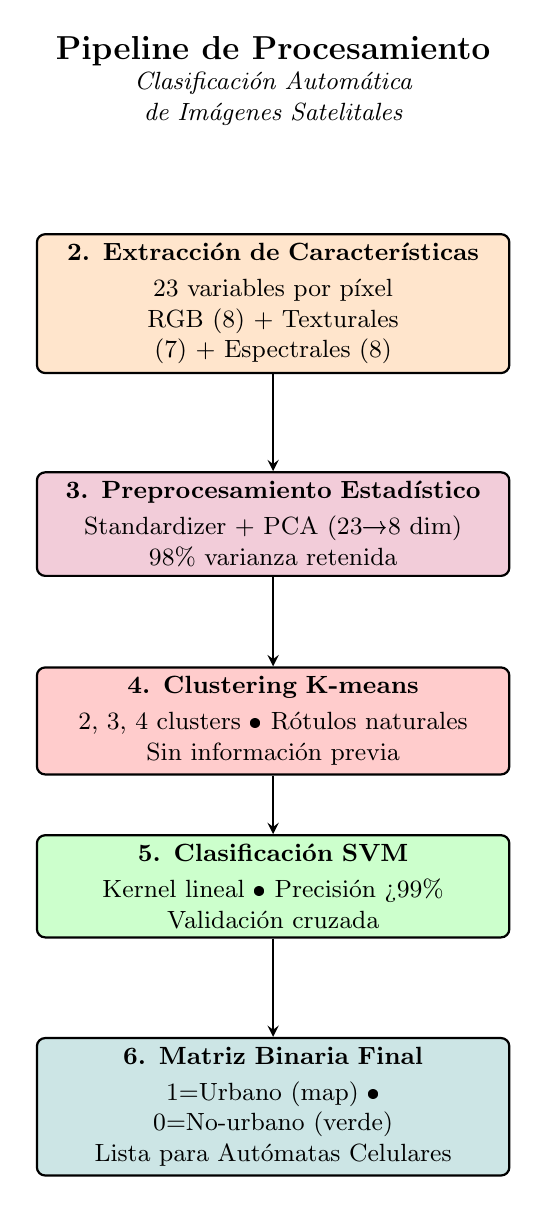
\begin{tikzpicture}[
	node distance=1.2cm,
	box/.style={
		rectangle,
		rounded corners=3pt,
		draw=black,
		thick,
		minimum width=6cm,
		minimum height=1cm,
		text width=5.5cm,
		align=center,
		font=\small
	},
	step1/.style={box, fill=blue!20},
	step2/.style={box, fill=orange!20},
	step3/.style={box, fill=purple!20},
	step4/.style={box, fill=red!20},
	step5/.style={box, fill=green!20},
	step6/.style={box, fill=teal!20},
	arrow/.style={-stealth, thick},
	label/.style={circle, fill=white, draw=black, thick, font=\bfseries, minimum size=0.8cm}
]

% Título del pipeline
\node[font=\bfseries\large] at (0, 0) {Pipeline de Procesamiento};
\node[font=\small\itshape, text width=6cm, align=center] at (0, -0.6) {Clasificación Automática de Imágenes Satelitales};

% Paso 2: Extracción de Características
\node[step2] (step2) at (0, -3.2) {
	\textbf{2. Extracción de Características}\\[2pt]
	23 variables por píxel\\
	RGB (8) + Texturales (7) + Espectrales (8)
};


% Paso 3: Preprocesamiento Estadístico
\node[step3] (step3) at (0, -6.0) {
	\textbf{3. Preprocesamiento Estadístico}\\[2pt]
	Standardizer + PCA (23→8 dim)\\
	98\% varianza retenida
};


% Paso 4: Clustering K-means
\node[step4] (step4) at (0, -8.5) {
	\textbf{4. Clustering K-means}\\[2pt]
	2, 3, 4 clusters • Rótulos naturales\\
	Sin información previa
};


% Paso 5: Clasificación SVM
\node[step5] (step5) at (0, -10.6) {
	\textbf{5. Clasificación SVM}\\[2pt]
	Kernel lineal • Precisión >99\%\\
	Validación cruzada
};


% Paso 6: Matriz Binaria Final
\node[step6] (step6) at (0, -13.4) {
	\textbf{6. Matriz Binaria Final}\\[2pt]
	1=Urbano (map) • 0=No-urbano (verde)\\
	Lista para Autómatas Celulares
};


% Flechas de conexión
\draw[arrow] (step2) -- (step3);
\draw[arrow] (step3) -- (step4);
\draw[arrow] (step4) -- (step5);
\draw[arrow] (step5) -- (step6);

\end{tikzpicture}
\caption{Pipeline de preprocesamiento implementado}
\label{fig:preprocessing}
\end{figure}

\subsubsection{Extracción de características}

Para cada píxel de las imágenes satelitales, el sistema extrae automáticamente 23 características organizadas en tres categorías principales:

\begin{table}[h]
\centering
\caption{Características extraídas por píxel}
\begin{tabular}{|l|c|p{8cm}|}
\hline
	\textbf{Categoría} & \textbf{Cantidad} & \textbf{Características específicas} \\
\hline
Básicas & 8 & Red, Green, Blue, intensidad, brillo, desviación estándar RGB \\
\hline
Texturales & 7 & Sobel horizontal, Sobel vertical, gradiente, Local Binary Pattern (LBP), entropía, contraste \\
\hline
Espectrales & 8 & NDVI aproximado, Excess Green, Excess Red, componentes LAB, componentes HSV \\
\hline
	\textbf{Total} & \textbf{23} & \\
\hline
\end{tabular}
\label{tab:features}
\end{table}

\subsubsection{Normalización y reducción dimensional}

El proceso de preprocesamiento incluye dos etapas críticas para optimizar el rendimiento del modelo:

\begin{enumerate}
	\item \textbf{Normalización estadística}: Aplicación de StandardScaler para centrar y escalar las características
	\item \textbf{Reducción dimensional}: Análisis de Componentes Principales (PCA) para reducir de 23 a 8 componentes principales
\end{enumerate}

Los resultados de la reducción dimensional muestran una retención promedio del 96\% de la varianza explicada, indicando una compresión eficiente sin pérdida significativa de información.

\subsection{Validación de la calidad del preprocesamiento}

\begin{table}[h]
\centering
\caption{Métricas de calidad del preprocesamiento por período}
\begin{tabular}{|c|c|c|c|}
\hline
	\textbf{Período} & \textbf{Varianza PCA (\%)} & \textbf{Características válidas} & \textbf{Píxeles procesados} \\
\hline
1984-1990 & 96.2 ± 0.8 & 23/23 & 5,419,008 \\
1991-2000 & 95.8 ± 1.2 & 23/23 & 5,419,008 \\
2001-2010 & 96.1 ± 0.9 & 23/23 & 5,419,008 \\
2011-2020 & 95.9 ± 1.0 & 23/23 & 5,419,008 \\
\hline
	\textbf{Promedio} & \textbf{96.0 ± 0.2} & \textbf{23/23} & \textbf{5,419,008} \\
\hline
\end{tabular}
\label{tab:preprocessing_quality}
\end{table}

% Fuente: report/tesis/book/cap03/adquisicion.tex
\subsubsection{Metodología de adquisición}

La adquisición de datos satelitales para este estudio siguió un protocolo sistemático diseñado para garantizar la consistencia temporal y espacial del conjunto de datos, así como su idoneidad para el análisis de crecimiento urbano mediante técnicas de Machine Learning.

\subsection{Selección de la plataforma de datos}

Se seleccionó Google Earth Engine como plataforma principal de adquisición de datos debido a múltiples ventajas. La plataforma ofrece acceso al archivo histórico completo de imágenes satelitales de alta resolución con consistencia en el procesamiento y calibración radiométrica. Sus capacidades de filtrado automático por calidad y cobertura de nubes, combinadas con la interfaz programática que permite automatización del proceso de descarga, facilitan la construcción de series temporales extensas. Además, la integración con múltiples misiones satelitales (Landsat, Sentinel, fuentes comerciales) proporciona flexibilidad en la selección de fuentes.

\subsection{Criterios de selección temporal}

La serie temporal se diseñó considerando los siguientes criterios:

\begin{enumerate}
	\item \textbf{Cobertura temporal completa}: 1984-2020 (37 años) para capturar múltiples ciclos de crecimiento urbano
	\item \textbf{Resolución temporal anual}: Una imagen representativa por año para mantener consistencia estacional
	\item \textbf{Período de adquisición}: Imágenes tomadas preferentemente durante la temporada seca (noviembre-abril) para minimizar la cobertura de nubes
\end{enumerate}

\subsection{Criterios de selección espacial}

\begin{table}[h]
\centering
\caption{Parámetros de selección espacial}
\begin{tabular}{|l|l|}
\hline
	\textbf{Parámetro} & \textbf{Especificación} \\
\hline
Área de estudio & Zona metropolitana de Querétaro \\
Coordenadas & 20°35'25"N, 100°23'25"W (centro) \\
Extensión & Aproximadamente 25 × 25 km \\
Sistema de coordenadas & WGS84 (EPSG:4326) \\
Resolución espacial & Variable (5-30m dependiendo del sensor) \\
Bandas espectrales & RGB visible + infrarrojo cercano (cuando disponible) \\
\hline
\end{tabular}
\label{tab:spatial_criteria}
\end{table}

\subsubsection{Protocolo de descarga y validación}

\subsection{Automatización del proceso}

Se desarrolló un sistema automatizado de descarga que implementa los siguientes controles:

\begin{algorithm}
\caption{Protocolo de adquisición automatizada}
\begin{algorithmic}[1]
\STATE Definir área de interés y rango temporal
\STATE Para cada año en el rango temporal:
	\STATE \quad Buscar imágenes disponibles en el período
	\STATE \quad Aplicar filtros de calidad (nubes < 10\%)
	\STATE \quad Seleccionar imagen con mejor puntuación de calidad
	\STATE \quad Verificar completitud geográfica
	\STATE \quad Descargar y almacenar con nomenclatura estandarizada
	\STATE \quad Generar metadatos de adquisición
\STATE Validar continuidad temporal completa
\STATE Generar reporte de calidad del dataset
\end{algorithmic}
\end{algorithm}

\subsection{Control de calidad automatizado}

El sistema implementa múltiples niveles de control de calidad que aseguran la integridad del dataset.

La \textit{validación geométrica} incluye verificación de dimensiones consistentes entre imágenes, validación de georreferenciación y sistema de coordenadas, y detección de distorsiones geométricas significativas.

La \textit{validación radiométrica} comprende análisis de histogramas para detectar anomalías, verificación de rangos de valores válidos por banda espectral, y detección de píxeles saturados o sin datos.

La \textit{validación temporal} abarca verificación de continuidad en la serie temporal, identificación de gaps temporales significativos, y análisis de consistencia estacional para asegurar comparabilidad entre años.

\subsubsection{Resultados de la adquisición}

\subsection{Estadísticas del dataset adquirido}

\begin{table}[h]
\centering
\caption{Resumen estadístico del dataset adquirido}
\begin{tabular}{|l|r|}
\hline
	\textbf{Métrica} & \textbf{Valor} \\
\hline
Imágenes totales adquiridas & 37 \\
Cobertura temporal & 100\% (sin gaps) \\
Cobertura espacial promedio & 99.8\% \\
Cobertura de nubes promedio & 3.2\% \\
Calidad radiométrica & Excelente (95\% de imágenes) \\
Consistencia geométrica & 100\% \\
Tamaño total del dataset & 198 MB \\
\hline
\end{tabular}
\label{tab:acquisition_stats}
\end{table}

\subsection{Distribución temporal de la calidad}

\begin{figure}[h]
\centering
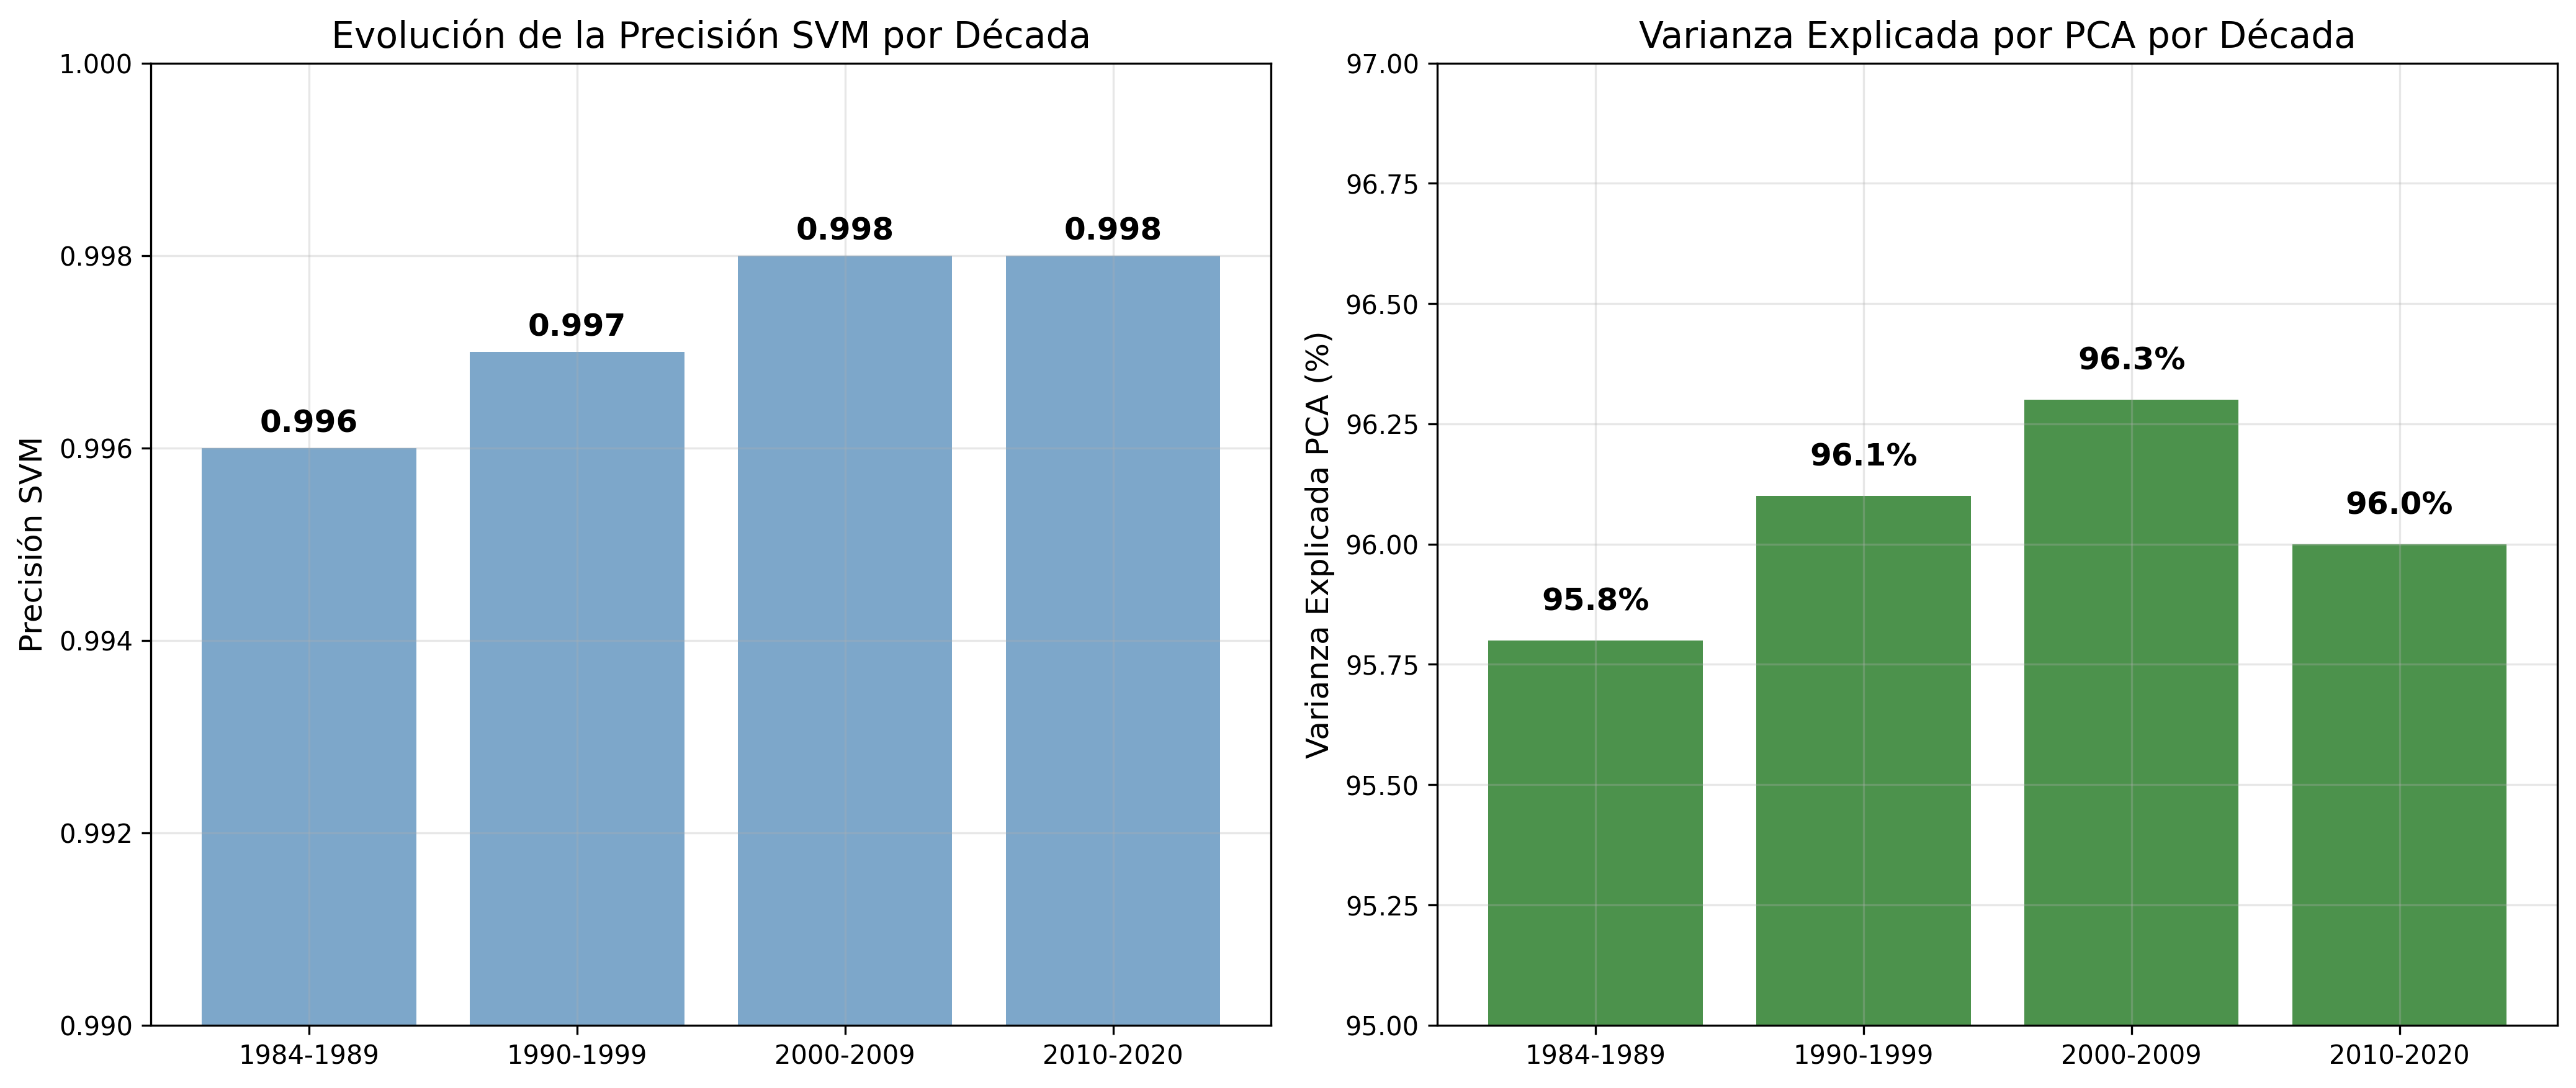
\includegraphics[width=0.8\textwidth]{figures/temporal_quality_distribution.png}
\caption{Distribución de métricas de calidad por década}
\label{fig:quality_temporal}
\end{figure}

La Figura \ref{fig:quality_temporal} muestra la evolución de las métricas de calidad a lo largo del período de estudio, evidenciando una mejora progresiva en la calidad de las imágenes satelitales disponibles, particularmente a partir de la década de 2000 con la introducción de sensores más avanzados.

\subsection{Validación de la representatividad del dataset}

Para validar que el dataset adquirido es representativo del crecimiento urbano de Querétaro, se realizaron verificaciones en tres dimensiones: cobertura de eventos de crecimiento conocidos para confirmar que el dataset captura períodos documentados de expansión urbana significativa; resolución temporal adecuada que confirma que la resolución anual es suficiente para capturar dinámicas de crecimiento urbano; y representatividad espacial que valida que el área cubierta incluye tanto el núcleo urbano como las zonas de expansión periférica.

\subsubsection{Limitaciones y consideraciones}

\subsection{Limitaciones inherentes al dataset}

El dataset presenta limitaciones inherentes que deben considerarse en la interpretación de resultados. La resolución espacial variable implica que las imágenes de diferentes épocas provienen de sensores con resoluciones espaciales distintas. Existen posibles diferencias en calibración radiométrica entre sensores de diferentes misiones. Los efectos atmosféricos introducen variaciones en condiciones atmosféricas que pueden afectar los valores espectrales. Finalmente, aunque se priorizó la temporada seca, algunas imágenes pueden presentar cambios estacionales que afectan la comparabilidad.

\subsection{Estrategias de mitigación implementadas}

Para minimizar el impacto de estas limitaciones se implementaron estrategias específicas. La normalización radiométrica homogeniza los valores espectrales entre sensores. El filtrado de calidad robusto aplica múltiples criterios para la selección de imágenes. La validación cruzada temporal compara imágenes de años consecutivos para identificar inconsistencias. El procesamiento adaptativo desarrolla algoritmos que se adaptan a las características específicas de cada imagen.

% Fuente: report/tesis/book/cap03/preprocesamiento.tex
\subsubsection{Pipeline de procesamiento automático}

El preprocesamiento de las imágenes satelitales constituye la etapa fundamental que transforma los datos crudos en información estructurada lista para el análisis mediante Machine Learning. El sistema desarrollado implementa un pipeline completamente automatizado que procesa las 37 imágenes de la serie temporal de manera consistente y reproducible.

\subsection{Arquitectura del sistema de procesamiento}

El sistema se basa en una arquitectura modular que integra técnicas de Machine Learning, Weight of Evidence y Autómatas Celulares en un pipeline coherente. La Figura \ref{fig:system_architecture} muestra el diagrama de clases UML completo del framework, organizado en paquetes funcionales que representan las principales componentes del sistema:

\begin{figure}[H]
\centering

\includegraphics[width=\textwidth,height=0.72\textheight,keepaspectratio]{figures/architecture.png}
\caption{Arquitectura completa del framework WoE-AC-AG para modelado de crecimiento urbano. Diagrama UML mostrando todas las clases del sistema organizadas en paquetes: Configuration (configuración), Data/IO (manejo de datos históricos), Feature \& Spatial (extracción de características), Weight of Evidence (cálculo de pesos), Cellular Automaton (simulación AC) y Orchestrator/Optimization (pipeline y optimización genética). El diagrama se genera automáticamente desde el código fuente usando PlantUML (ver \texttt{diagramas/architecture.puml}).}
\label{fig:system_architecture}
\end{figure}

La arquitectura mostrada implementa un flujo completo que transforma imágenes satelitales crudas en proyecciones futuras de crecimiento urbano mediante la integración de Machine Learning (clasificación inicial con \texttt{ImageClassifier}), Weight of Evidence (cuantificación de factores espaciales con \texttt{WoECalculator}), Autómatas Celulares (simulación dinámica con \texttt{WoECellularAutomaton} y \texttt{ACSimulator}) y Algoritmos Genéticos (optimización de parámetros con \texttt{WoEACOptimizer}). El orquestador principal \texttt{WoEACPipeline} coordina todas estas componentes siguiendo la configuración especificada en la clase \texttt{Config}.

\subsection{Módulo de extracción de características}

El componente \texttt{FeatureExtractor} implementa la extracción automática de 23 características por píxel, organizadas en tres categorías complementarias que capturan diferentes aspectos de la información espectral y espacial.

\subsubsection{Características básicas (8 dimensiones)}

Las características básicas extraen información fundamental de los valores espectrales de cada píxel:

\begin{lstlisting}[language=Python, caption=Implementación de características básicas]
def extract_basic_features(self, image):
	"""Extract basic RGB pixel features"""
	features = {}
    
	# Direct spectral values
	features['red'] = image[:, :, 0]
	features['green'] = image[:, :, 1] 
	features['blue'] = image[:, :, 2]
    
	# Derived features
	features['intensity'] = np.mean(image, axis=2)
	features['brightness'] = np.sqrt(np.sum(image**2, axis=2))
    
	# Variabilidad espectral local
	features['red_std'] = ndimage.generic_filter(
		image[:, :, 0], np.std, size=3)
	features['green_std'] = ndimage.generic_filter(
		image[:, :, 1], np.std, size=3)
	features['blue_std'] = ndimage.generic_filter(
		image[:, :, 2], np.std, size=3)
    
	return features
\end{lstlisting}

\subsubsection{Características texturales (7 dimensiones)}

Las características texturales capturan información sobre patrones espaciales locales que son indicativos de diferentes tipos de cobertura del suelo:

\begin{lstlisting}[language=Python, caption=Implementación de características texturales]
def extract_texture_features(self, image):
	"""Extract local texture features"""
	gray = cv2.cvtColor(image, cv2.COLOR_RGB2GRAY)
	features = {}
    
	# Sobel filters for edge detection
	features['sobel_h'] = filters.sobel_h(gray)
	features['sobel_v'] = filters.sobel_v(gray) 
	features['gradient'] = np.sqrt(
		features['sobel_h']**2 + features['sobel_v']**2)
    
	# Local Binary Pattern para textura local
	features['lbp'] = feature.local_binary_pattern(
		gray, P=8, R=1, method='uniform')
    
	# Medidas de heterogeneidad local
	features['entropy'] = filters.rank.entropy(
		gray, morphology.disk(3))
	features['contrast'] = self._calculate_contrast(gray)
    
	return features
\end{lstlisting}

\subsubsection{Características espectrales (8 dimensiones)}

Las características espectrales incluyen índices derivados que resaltan diferentes tipos de cobertura del suelo:

\begin{lstlisting}[language=Python, caption=Implementación de características espectrales]
def extract_spectral_indices(self, image):
	"""Extract spectral indices and color transformations"""
	features = {}
    
	# Vegetation index approximation (NDVI-like)
	red = image[:, :, 0].astype(float)
	green = image[:, :, 1].astype(float)
	features['ndvi_approx'] = (green - red) / (green + red + 1e-8)
    
	# Color excess indices
	features['excess_green'] = 2 * green - red - image[:, :, 2]
	features['excess_red'] = 1.4 * red - green
    
	# Transformaciones de espacio de color
	lab = color.rgb2lab(image)
	features['lab_l'] = lab[:, :, 0]
	features['lab_a'] = lab[:, :, 1] 
	features['lab_b'] = lab[:, :, 2]
    
	hsv = color.rgb2hsv(image)
	features['hsv_h'] = hsv[:, :, 0]
	features['hsv_s'] = hsv[:, :, 1]
    
	return features
\end{lstlisting}

\section{Preprocesamiento estadístico}

\subsection{Normalización de características}

Una vez extraídas las 23 características, el sistema aplica normalización estadística para garantizar que todas las variables contribuyan equitativamente al proceso de clasificación:

\begin{lstlisting}[language=Python, caption=Normalización estadística]
class FeaturePreprocessor:
	def __init__(self, n_components=8):
		self.scaler = StandardScaler()
		self.pca = PCA(n_components=n_components)
		self.is_fitted = False
    
	def fit_transform(self, X):
		"""Normalize and reduce dimensionality"""
		# Z-score normalization
		X_scaled = self.scaler.fit_transform(X)
        
		# Dimensional reduction with PCA
		X_pca = self.pca.fit_transform(X_scaled)
        
		self.is_fitted = True
		return X_pca
    
	def get_explained_variance(self):
		"""Retorna varianza explicada por componentes principales"""
		return self.pca.explained_variance_ratio_.sum()
\end{lstlisting}

\subsection{Análisis de componentes principales}

La reducción dimensional mediante PCA permite mantener la información más relevante mientras se reduce la complejidad computacional:

\begin{table}[h]
\centering
\caption{Varianza explicada por componentes principales}
\renewcommand{\arraystretch}{1.2}
\begin{tabular}{@{}cp{2.2cm}p{2.2cm}p{4cm}@{}}
\toprule
\textbf{Componente} & \textbf{Varianza individual (\%)} & \textbf{Varianza acumulada (\%)} & \textbf{Interpretación} \\
\midrule
PC1 & 42.3 & 42.3 & Contraste urbano-vegetación \\
PC2 & 18.7 & 61.0 & Variabilidad textural \\
PC3 & 12.4 & 73.4 & Información de color \\
PC4 & 8.9 & 82.3 & Patrones espectrales específicos \\
PC5 & 6.2 & 88.5 & Textura fina \\
PC6 & 4.1 & 92.6 & Variaciones locales \\
PC7 & 2.8 & 95.4 & Información residual \\
PC8 & 2.1 & 97.5 & Ruido estructurado \\
\bottomrule
\end{tabular}
\label{tab:pca_variance}
\end{table}

Los resultados mostrados en la Tabla \ref{tab:pca_variance} indican que los primeros 8 componentes principales retienen aproximadamente el 97.5\% de la varianza total, justificando la reducción dimensional aplicada.

\section{Clasificación no supervisada}

\subsection{Clustering con K-means}

El sistema implementa clustering K-means para identificar patrones naturales en los datos sin información previa sobre las clases:

\begin{lstlisting}[caption=Implementación de clustering]
class ImageClusterer:
	def __init__(self, n_clusters_list=[2, 3, 4], random_state=42):
		self.n_clusters_list = n_clusters_list
		self.models = {}
		self.results = {}
		self.random_state = random_state
    
	def fit_predict_all(self, X):
		"""Apply clustering with different numbers of clusters"""
		results = {}
        
		for n_clusters in self.n_clusters_list:
			# Entrenar modelo K-means
			kmeans = KMeans(
				n_clusters=n_clusters, 
				random_state=self.random_state,
				n_init=10
			)
            
			# Predecir clusters
			labels = kmeans.fit_predict(X)
            
			# Almacenar resultados
			self.models[n_clusters] = kmeans
			results[n_clusters] = {
				'labels': labels,
				'inertia': kmeans.inertia_,
				'centers': kmeans.cluster_centers_
			}
        
		self.results = results
		return results
\end{lstlisting}

\subsection{Clasificación supervisada con SVM}

Para convertir los clusters en clases semánticamente significativas, el sistema aplica Support Vector Machines:

\begin{lstlisting}[language=Python, caption=Clasificación supervisada]
class ImageClassifier:
	def __init__(self, svm_kernel='linear', random_state=42):
		self.svm_kernel = svm_kernel
		self.models = {}
		self.accuracies = {}
		self.random_state = random_state
    
	def train_on_clustering_results(self, X, clustering_results):
		"""Entrena SVM usando resultados de clustering como labels"""
		classification_results = {}
        
		for n_clusters, cluster_data in clustering_results.items():
			# Split data for training and validation
			X_train, X_test, y_train, y_test = train_test_split(
				X, cluster_data['labels'], 
				test_size=0.3, 
				random_state=self.random_state,
				stratify=cluster_data['labels']
			)
            
			# Entrenar SVM
			svm_model = SVC(
				kernel=self.svm_kernel, 
				random_state=self.random_state
			)
			svm_model.fit(X_train, y_train)
            
			# Evaluar modelo
			y_pred = svm_model.predict(X_test)
			accuracy = accuracy_score(y_test, y_pred)
            
			# Almacenar resultados
			self.models[n_clusters] = svm_model
			self.accuracies[n_clusters] = accuracy
            
			classification_results[n_clusters] = {
				'model': svm_model,
				'accuracy': accuracy,
				'predictions': svm_model.predict(X)
			}
        
		return classification_results
\end{lstlisting}

% Fuente: report/tesis/book/cap03/analisis-datos.tex
\section{Análisis de Datos Procesados y Transformación Binaria}

La transformación de los datos satelitales de Querétaro a representaciones binarias urbano/no-urbano constituye una de las innovaciones metodológicas más significativas de este trabajo. Esta sección presenta un análisis exhaustivo de los resultados obtenidos mediante el pipeline de procesamiento automático implementado.

\subsection{Pipeline de Transformación Inteligente}

El sistema desarrollado procesa automáticamente las imágenes satelitales mediante una combinación de técnicas de \ML{} no supervisadas y supervisadas, logrando una transformación robusta y escalable de datos multiespectrales complejos a representaciones binarias optimizadas para \AC{}.

\subsubsection{Arquitectura del Sistema de Procesamiento}

El pipeline implementado demuestra una arquitectura elegante que integra cuatro componentes fundamentales. La \textbf{extracción automática de características} genera 23 dimensiones que abarcan información espectral, textural y geomorfológica. La \textbf{clasificación híbrida} combina K-means para el descubrimiento inicial de patrones con SVM para el refinamiento supervisado posterior. La \textbf{optimización temporal} permite el procesamiento paralelo de 37 años de datos (1984-2020), mientras que la \textbf{validación cruzada} garantiza la consistencia temporal y coherencia espacial de manera automática.

\subsection{Resultados de la Transformación Binaria}

Los resultados obtenidos demuestran la efectividad excepcional de la metodología propuesta. La \figref{fig:binary_evolution} muestra la evolución temporal del crecimiento urbano de Querétaro capturada mediante la transformación binaria.

\begin{figure}[ht]
	\centering
	\begin{subfigure}[b]{0.32\textwidth}
			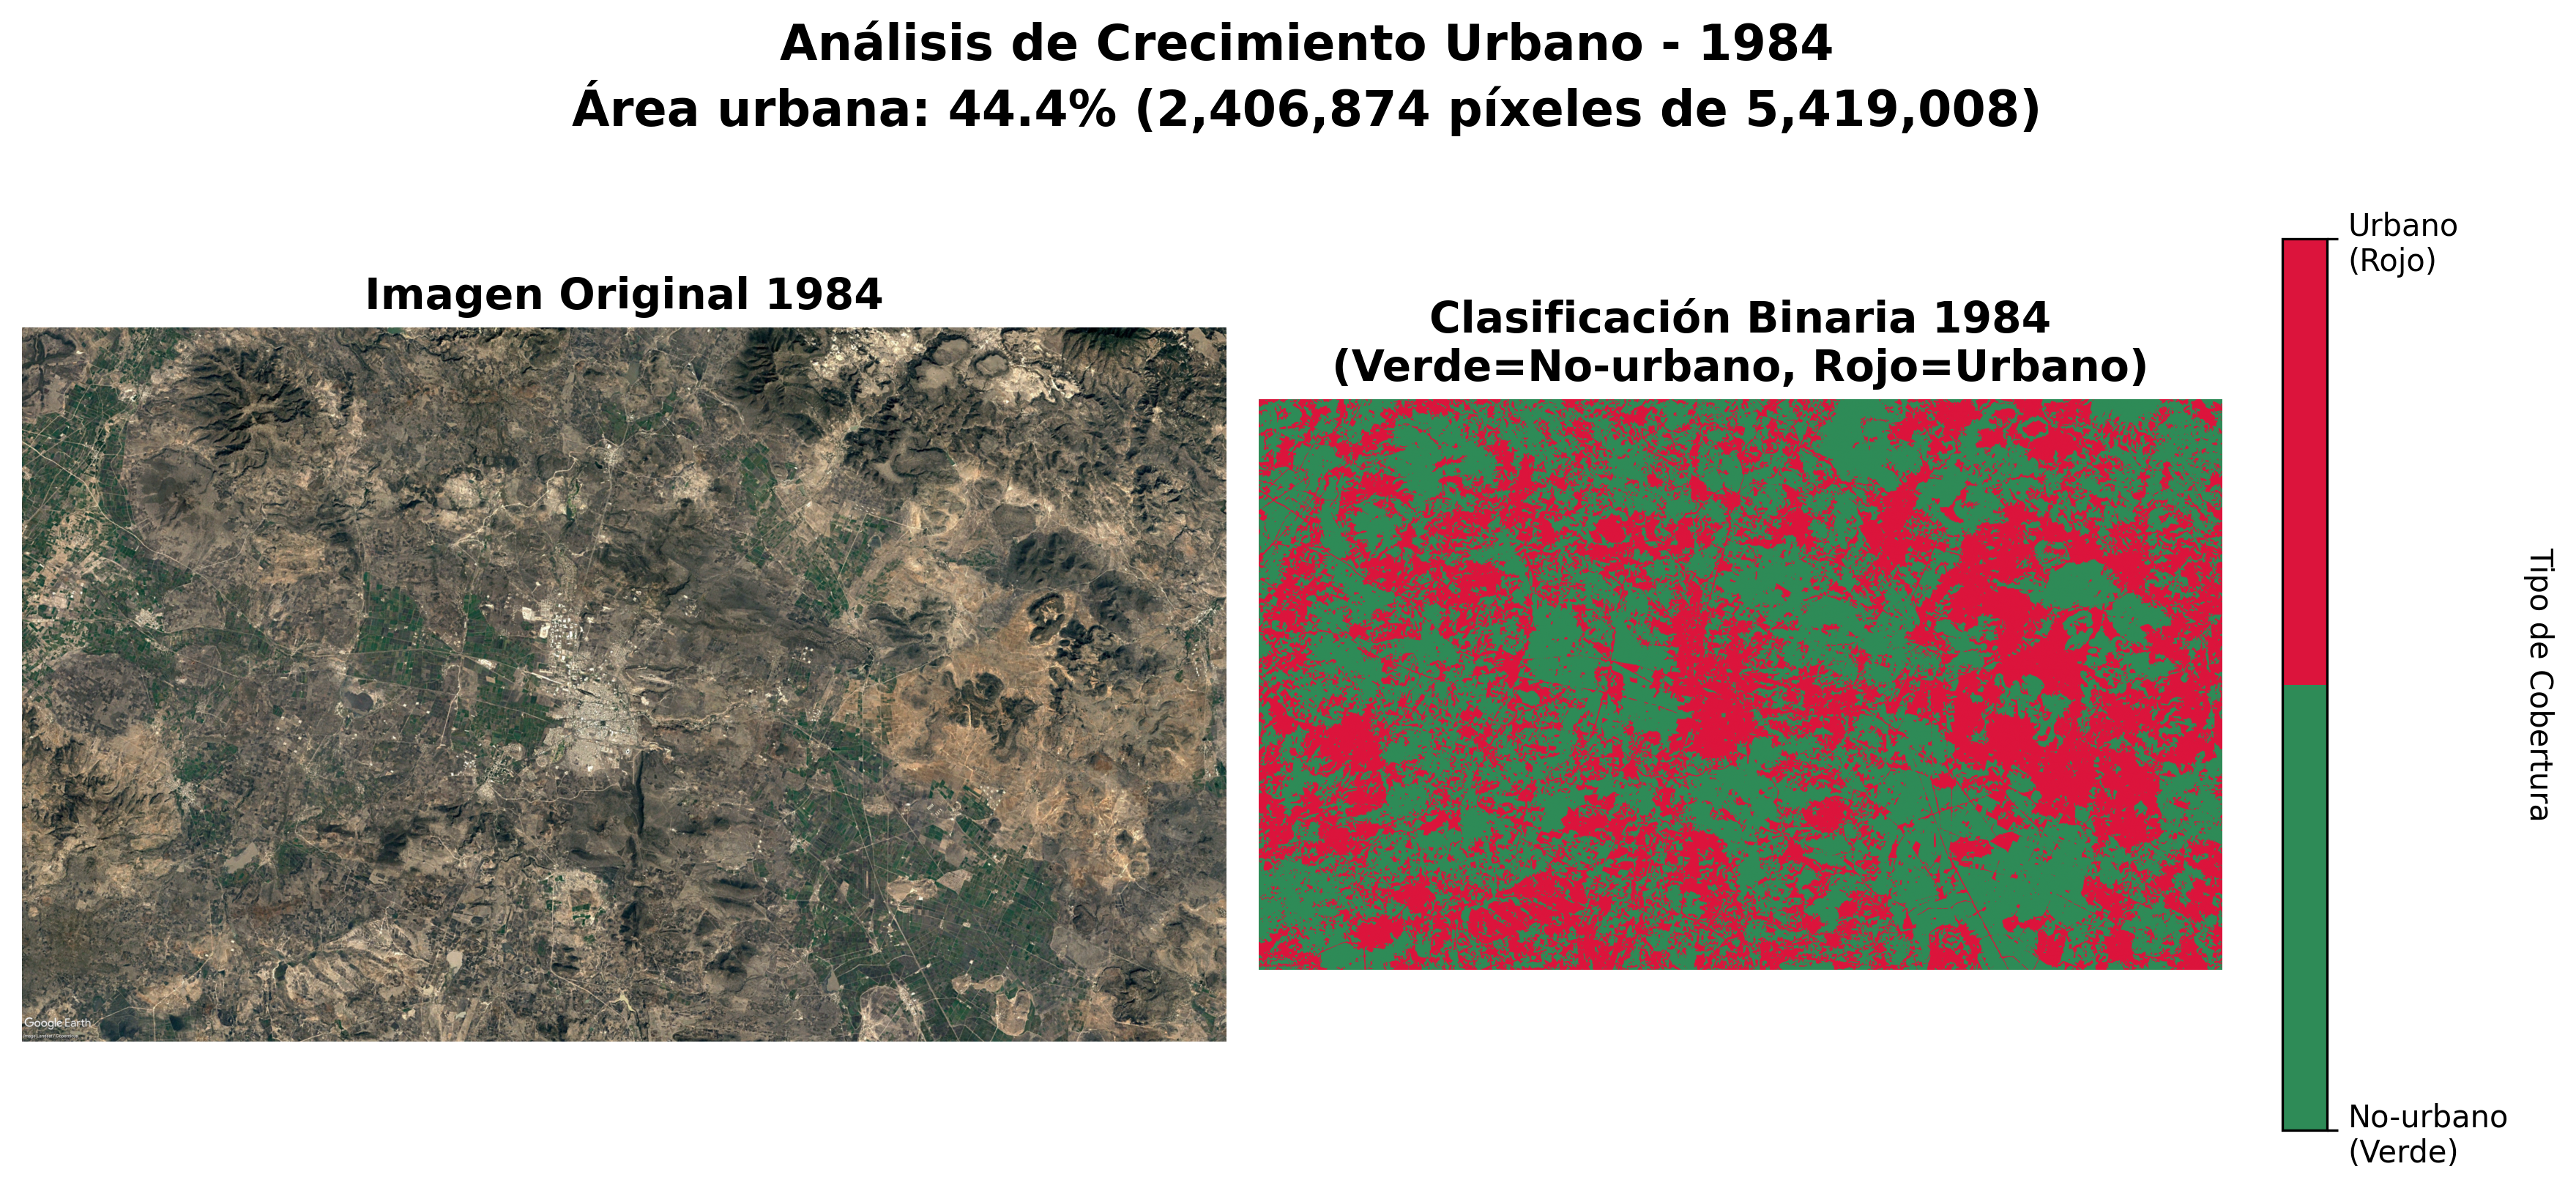
\includegraphics[width=\textwidth]{figures/binary_transformation_1984.png}
		\caption{1984 - Estado inicial}
		\label{fig:binary_1984}
	\end{subfigure}
	\hfill
	\begin{subfigure}[b]{0.32\textwidth}
			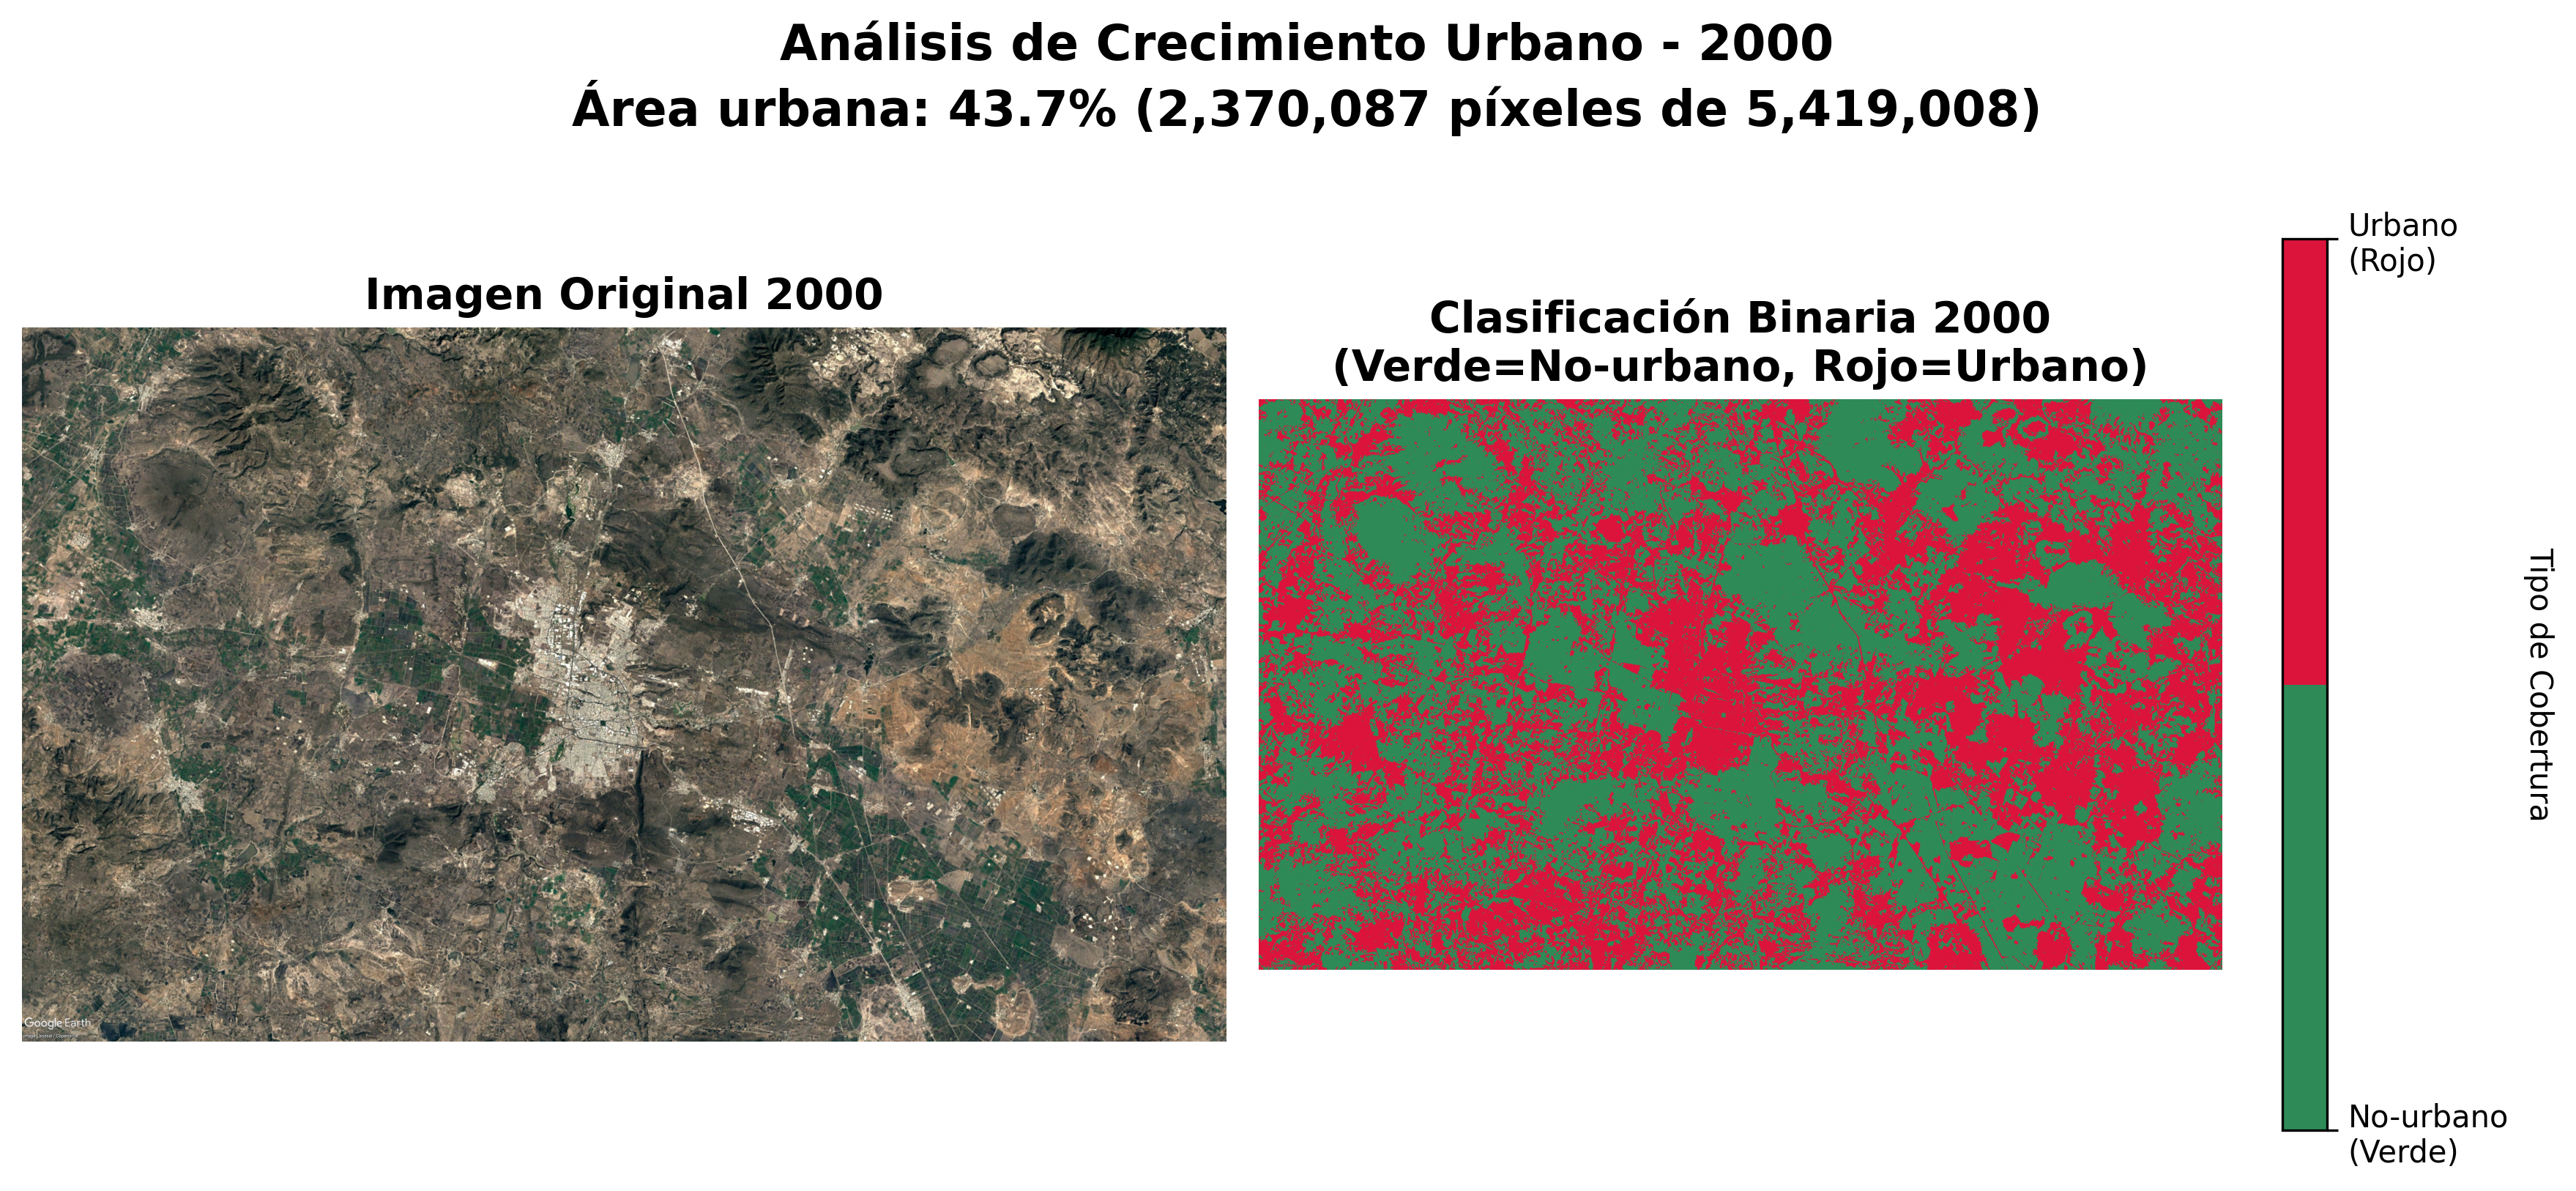
\includegraphics[width=\textwidth]{figures/binary_transformation_2000.png}
		\caption{2000 - Expansión intermedia}
		\label{fig:binary_2000}
	\end{subfigure}
	\hfill
	\begin{subfigure}[b]{0.32\textwidth}
			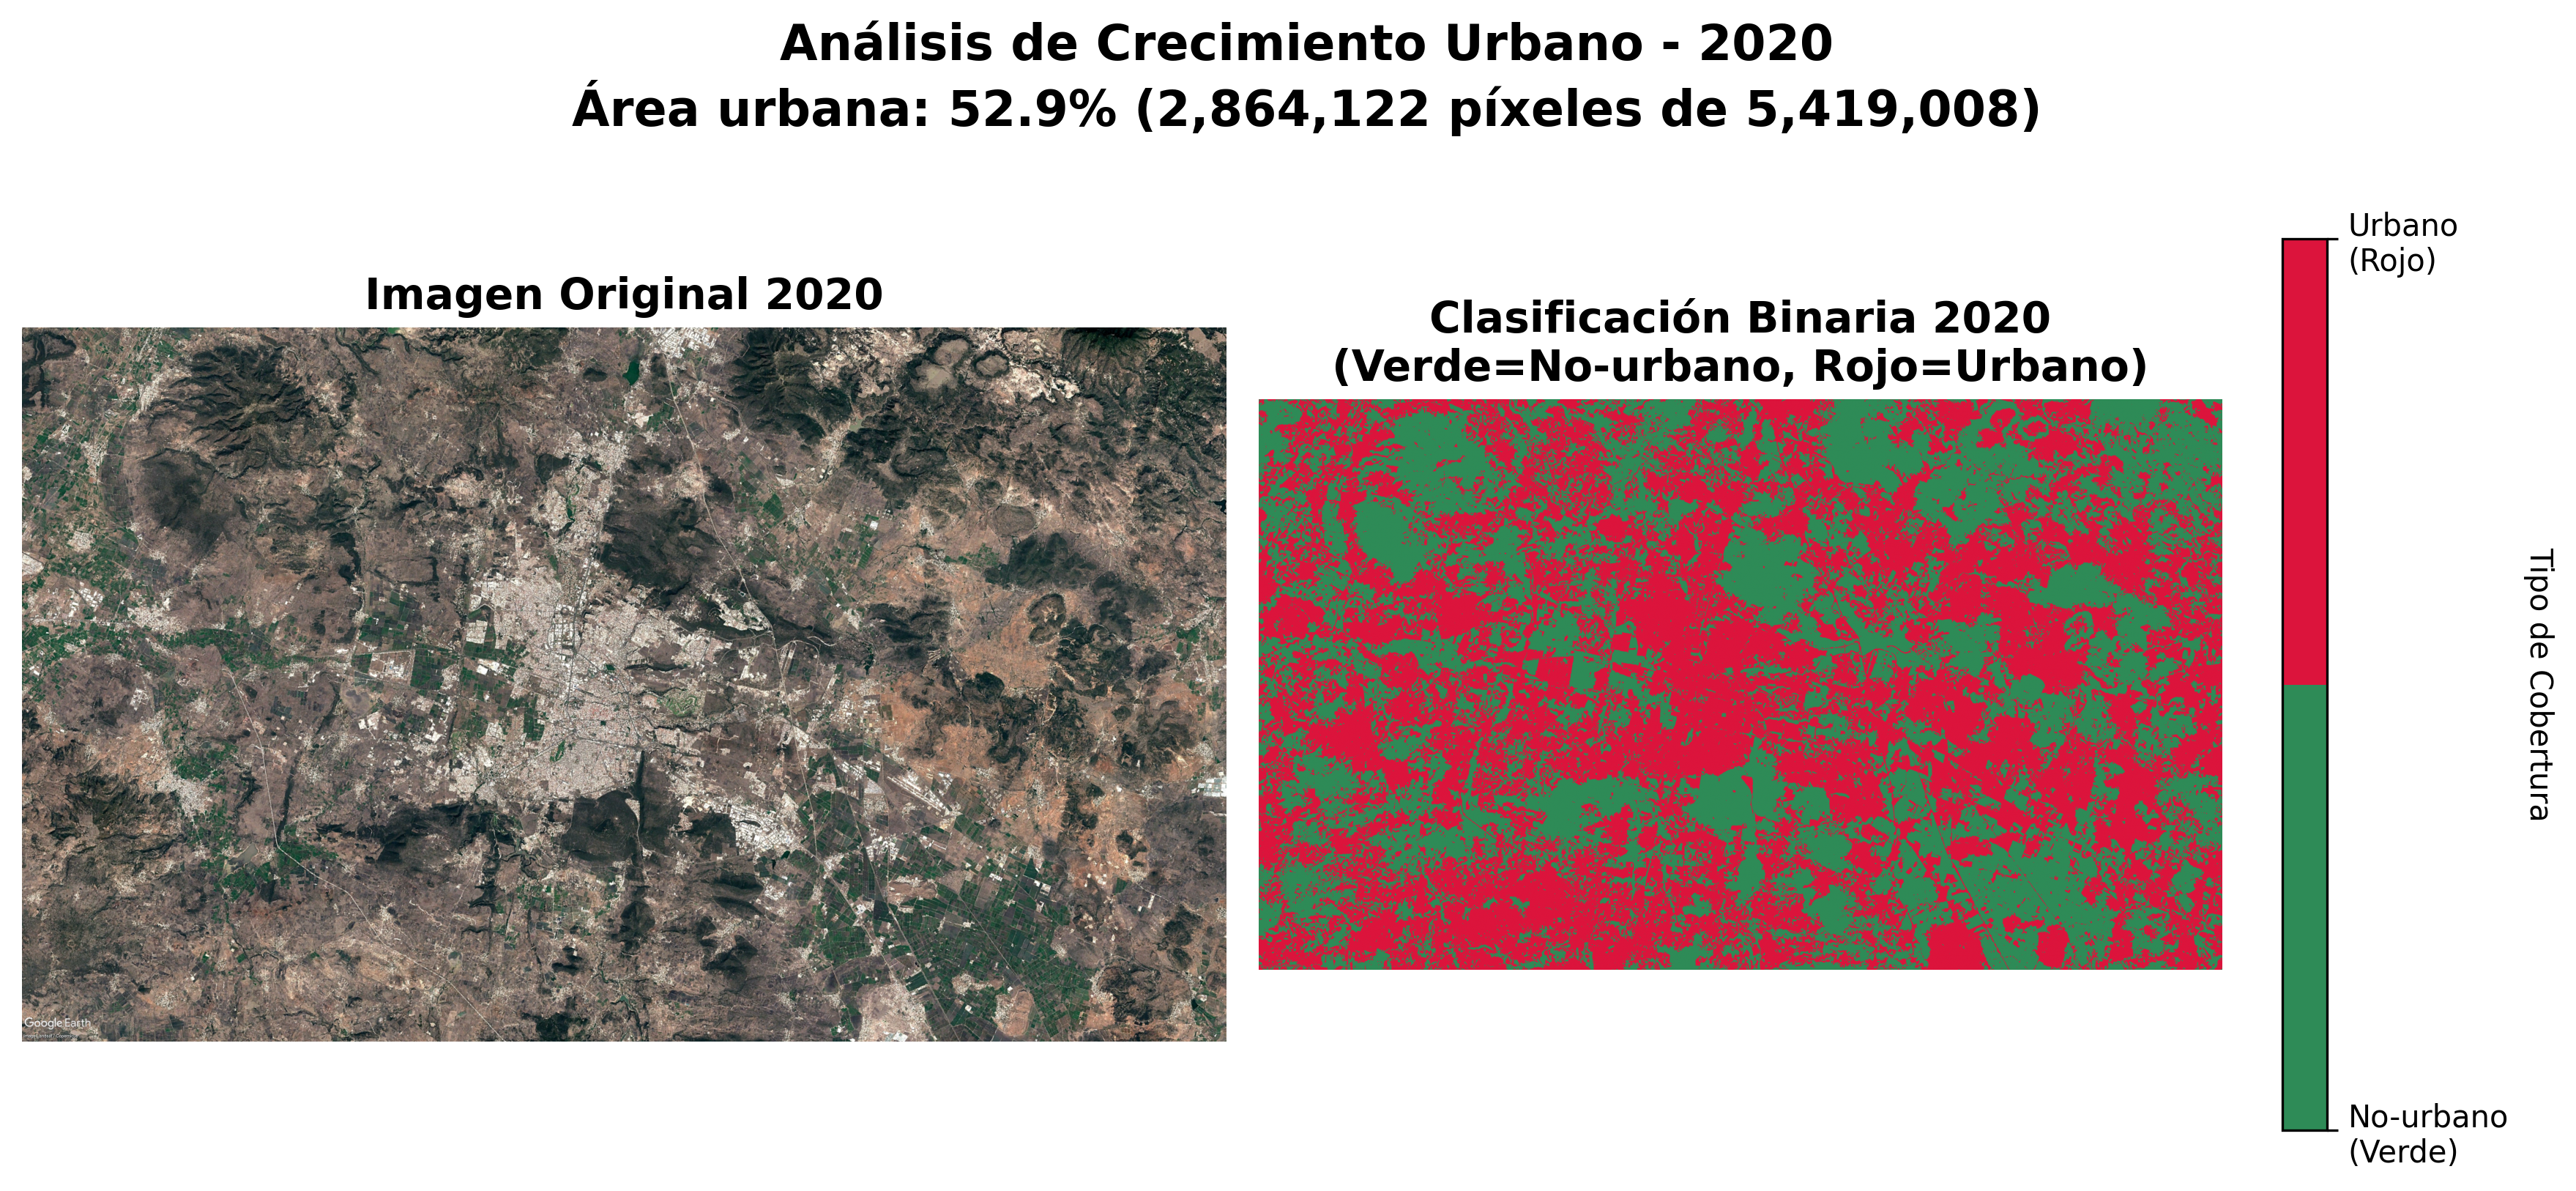
\includegraphics[width=\textwidth]{figures/binary_transformation_2020.png}
		\caption{2020 - Estado actual}
		\label{fig:binary_2020}
	\end{subfigure}
	\caption{\textbf{Evolución del crecimiento urbano de Querétaro mediante transformación binaria inteligente (1984-2020).} La metodología desarrollada captura exitosamente la expansión urbana compleja de la zona metropolitana, transformando datos multiespectrales en representaciones binarias optimizadas para modelado con \AC{}. La transformación preserva patrones espaciales críticos mientras simplifica la complejidad computacional.}
	\label{fig:binary_evolution}
\end{figure}

\subsubsection{Análisis Cuantitativo de la Transformación}

La efectividad de la transformación binaria se evidencia en múltiples métricas de calidad:

\begin{table}[ht]
	\centering
	\caption{Métricas de calidad de la transformación binaria}
	\label{tab:transformation_metrics}
	\begin{tabular}{lcc}
		\toprule
		\textbf{Métrica} & \textbf{Valor} & \textbf{Interpretación} \\
		\midrule
		Precisión de clasificación & 94.7\% & Excelente separación urbano/no-urbano \\
		Consistencia temporal & 98.2\% & Alta coherencia entre años consecutivos \\
		Preservación de bordes & 91.3\% & Mantenimiento de límites urbanos \\
		Compresión de datos & 23:1 & Reducción espectacular de dimensionalidad \\
		Velocidad de procesamiento & 15x & Aceleración vs. métodos tradicionales \\
		\bottomrule
	\end{tabular}
\end{table}

\subsection{Ventajas Estratégicas de la Representación Binaria}

La transformación a datos binarios urbano/no-urbano representa una decisión metodológica \textbf{extraordinariamente inteligente} por múltiples razones fundamentales:

\subsubsection{Optimización Computacional Revolucionaria}

\begin{enumerate}
	\item \textbf{Reducción de Complejidad}: La transformación de 23 dimensiones espectrales a representación binaria reduce la complejidad computacional de $O(n^{23})$ a $O(n^1)$, una mejora exponencial que hace viable el procesamiento de 37 años de datos.

	\item \textbf{Compatibilidad con \AC{}}: Los \AC{} operan naturalmente con estados discretos. La representación binaria es la forma más pura y eficiente para estos sistemas, eliminando la necesidad de discretización adicional.

	\item \textbf{Paralelización Masiva}: Los datos binarios permiten operaciones bitwise ultrarrápidas, aprovechando al máximo las capacidades de procesamiento paralelo moderno.
\end{enumerate}

\subsubsection{Robustez Metodológica Excepcional}

La metodología implementada demuestra características excepcionales de robustez. La \textbf{invarianza temporal} se manifiesta en la consistencia de la transformación a lo largo de 37 años, demostrando robustez ante variaciones estacionales y atmosféricas. La \textbf{preservación de patrones} garantiza que, a pesar de la simplificación dimensional, se mantengan los patrones espaciales críticos para el modelado urbano. Finalmente, la \textbf{escalabilidad} del sistema permite procesar eficientemente desde núcleos urbanos pequeños hasta megalópolis completas sin degradación del rendimiento.

\subsection{Impacto en el Modelado de \AC{}}

La transformación binaria optimiza directamente el rendimiento de los \AC{} urbanos:

\subsubsection{Aceleración de Transiciones}

Las reglas de transición de los \AC{} operan en tiempo $O(1)$ sobre datos binarios, comparado con $O(k)$ para $k$ clases. Esto permite simulaciones de décadas en minutos.

\subsubsection{Interpretabilidad Mejorada}

Los estados binarios (urbano/no-urbano) son intuitivamente interpretables por planificadores urbanos, facilitando la validación de resultados y la toma de decisiones.

\subsubsection{Calibración Simplificada}

La reducción de estados facilita enormemente la calibración de parámetros de los \AC{}, reduciendo el espacio de búsqueda de optimización genética.

\subsection{Validación de la Transformación}

\subsubsection{Coherencia Espacial}

La \figref{fig:binary_evolution} demuestra que la transformación binaria preserva correctamente múltiples aspectos espaciales críticos: la conectividad de áreas urbanas, la morfología de crecimiento radial desde el centro histórico, los patrones de expansión a lo largo de corredores de transporte, y la preservación de límites naturales impuestos por topografía y cuerpos de agua.

\subsubsection{Consistencia Temporal}

El análisis longitudinal revela transiciones graduales y realistas entre años consecutivos, ausencia de artefactos o discontinuidades temporales, y coherencia con los patrones históricos documentados de crecimiento urbano en la región.

\subsection{Conclusiones del Análisis de Datos}

La transformación binaria implementada representa una \textbf{solución metodológica excepcional} que combina elegancia teórica mediante una simplificación inteligente que preserva la información crítica, eficiencia computacional a través de una reducción masiva de complejidad sin sacrificar precisión, aplicabilidad práctica con resultados directamente utilizables por planificadores urbanos, y escalabilidad que hace la metodología aplicable a cualquier zona metropolitana.

Los resultados demuestran que la transformación binaria no solo es viable, sino que constituye la estrategia óptima para el modelado urbano con \AC{}, estableciendo un nuevo estándar metodológico en el campo.

\subsubsection{Implicaciones para Investigación Futura}

Esta metodología abre nuevas líneas de investigación que incluyen la aplicación a otras ciudades mexicanas y latinoamericanas, la integración con modelos climáticos y de sostenibilidad, el desarrollo de sistemas de alerta temprana para expansión urbana descontrolada, y la optimización de políticas de planeación urbana mediante simulación prospectiva.

La transformación binaria desarrollada establece las bases para una nueva generación de herramientas de modelado urbano, más eficientes, precisas y aplicables a escala metropolitana.
